\subsection{Construcción de interfaces de usuario usando el patrón MVC}

	\subsubsection{MVC}
	El patrón \emph{Modelo-Vista-Controlador} (MVC) es una forma de construir
	interfaces de usuario (UI) que propone dividir el comportamiento de una
	aplicación en tres partes \cite{reenskaug79}:
		\begin {itemize}
		\item {\bf Modelo}
			El modelo representa nuestra percepción del mundo real. 
			Maneja el comportamiento y la información del dominio de la aplicación,
			responde a los pedidos de información sobre su estado y tiene la
			responsabilidad última de llevar a cabo el comportamiento del sistema.
			
		\item {\bf Vista}
			La vista tiene la responsabilidad de interactuar con el usuario, es la
			parte más fácil de identificar ya que es la que vemos en pantalla.
			La comunicación con el usuario es bidireccional:
			por un lado le muestra información proveniente del modelo y el otro lado
			recibe acciones de parte del usuario, que representa internamente como eventos.
			
		\item {\bf Controlador}
			Es el intermediario entre el modelo y la vista.
			Captura los eventos emanados de ambos y coordina la interacción entre los
			dos.
	\end {itemize}
	 
	La idea principal de MVC, y que influyó a la mayoría de los frameworks de
	presentación posteriores, es la de Presentación Separada \emph{(Separated
	Presentation)} \cite{burbeck87}.
	Esto nos brinda una clara separación de responsabilidades entre interfaz,
	lógica de negocio y control. Además nos permite soportar múltiples
	presentaciones para un mismo modelo de información.
	La figura \ref{mvc} muestra las relaciones entre los tres componentes.  
	
	\begin{figure}[h]
		\centering
		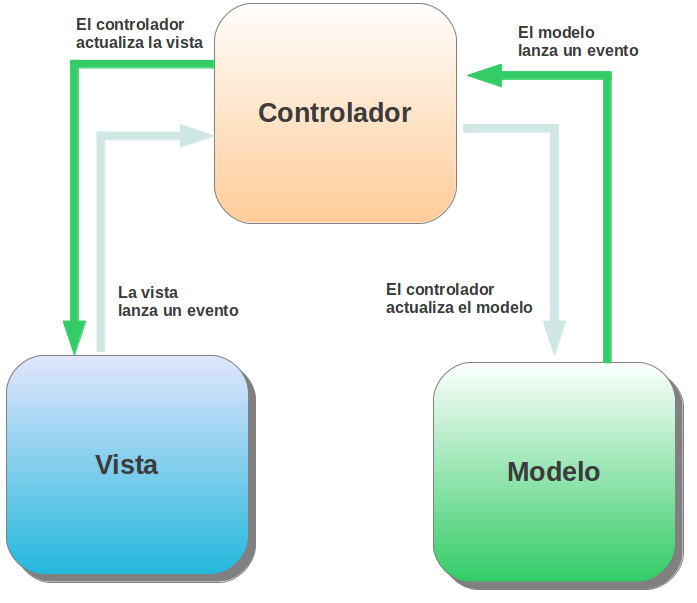
\includegraphics[width=300px, height=300px]{img/mvc} 
		\caption{Esquema MVC}
		\label{mvc}
	\end{figure}  
	
\subsubsection{Eventos}
\label{Eventos}

		Un evento es un suceso en el sistema, como una interacción del usuario con
	la máquina, o un cambio en el estado interno de un objeto.
	En un sistema orientado a eventos, existen fuentes que producen eventos y
	\emph{listeners} que se registran para ser notificados de esos eventos y poder
	actuar en consecuencia.	
	El patrón \emph{Observer} \cite{Gamma1995} es una forma común de implementar la
	idea de evento en lenguajes orientados a objetos.
	
	\begin{quote}
	
	\begin{description}
	   
	\item [Objetivo] Definir una dependencia 1:n de forma que cuando el objeto
		1 cambie su estado, los n objetos sean notificados y se actualicen
		automáticamente, a estos objetos se los conoce como \emph{listener}. Esto me
		permite una comunicación entre objetos con muy bajo acoplamiento.
	
	\item [Motivación] En la construcción de interfaces de usuarios, se tiende
		a separar los objetos de presentación (vistas) de los objetos de dominio, de
		forma que se puedan tener varias vistas sincronizadas de la misma información.
	
	\end{description}
	\end{quote}
	
\subsubsection{Binding}
\label{binding}

	El \emph{binding} es una conección de propiedades entre dos objetos, que
	permite mantener sincronizado el valor de una propiedad en el primero de esos
	objetos con el valor alguna propiedad del segundo objeto.
	Habitualmente esto se logra a través del uso de eventos.
	
	En la construcción de interfaces de usuario es habitual utilizar el concepto de
	binding para sincronizar los datos que está viendo o modificando el usuario
	con la información contenida en el modelo.
	Cada vez que el usuario ingresa o modifica un valor en la pantalla, la
	vista dispara un evento indicando el cambio de ese valor. Todas las
	propiedades del modelo que estén conectadas con esa propiedad, serán
	actualizadas automáticamente, dando la posibilidad de validar la información.
	En caso que las dos propiedades no sean del mismo tipo, el binding provee
	estrategias para realizar las conversiones que fueran necesarias.

	
	A continuación en la figura \ref{fig:binding} se describe el esquema de
		\emph{binding}
		
		\begin{figure}[h]
			\centering
			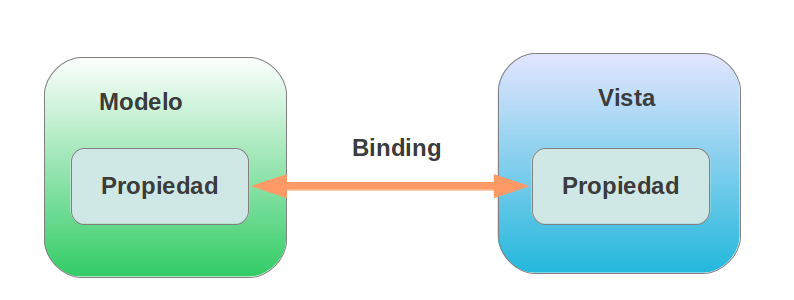
\includegraphics[width=300px]{img/binding}
			\caption{Esquema Binding}
			\label{fig:binding}
		\end{figure}
		
		\bigskip
	
	La ausencia de \emph{binding} implica mayor trabajo  y como consecuencia
	conlleva mayor tiempo de desarrollo en  traspasar la información de los
	objetos de dominio hacia los componentes de la interfaz gráfica y viceversa, repitiendo muchas lineas de código.
	
	Podemos tener información inconsistente, como por ejemplo, al mostrarse la interfaz,
	muestra el valor actual de la propiedad de un objeto de dominio, y después el
	objeto de dominio cambia el valor de su propiedad, la interfaz no se actualiza,
	y la información queda inconsistente.
	
	\bigskip
	
	Se pueden diferenciar dos tipos de \emph{binding}:
	
	\begin {itemize}
	
		\item {\bf Unidireccional}
		El \emph{binding} unidireccional permite que los cambios en la propiedad de
		origen (modelo) actualicen automáticamente la propiedad de destino (vista),
		pero los cambios en la propiedad del modelo no se propagan de nuevo a la
		propiedad de la vista.
		Este tipo de \emph{binding} es adecuado si el control que se va a enlazar es
		de sólo lectura de forma implícita.		
		
		\item {\bf Bidireccional}
		El \emph{binding} bidireccional permite que los cambios realizados en la
		propiedad del modelo o de la vista se actualicen automáticamente en el
		otro. Este tipo de \emph{binding} es adecuado para formularios modificables u
		otros escenarios de interfaz de usuario totalmente interactivos.
		Esto es posible, gracias a la utilización de los eventos, tanto desde el
		dominio como de la interfaz.
	
		En nuestro trabajo nos enfocamos en este tipo de binding.
		 
	
	\end {itemize}
	


\paragraph{Limitaciones}
	Para poder utilizar el \emph{binding}, se necesita que los objetos de dominio, 
	conozcan el concepto de eventos.
	
	Otro problema que aparece frecuentemente es que el binding en su versión más 
	sencilla modifica los objetos directamente, por lo que al cancelar una operación 
	se debe volver al estado anterior, y este proceso es repetitivo y propenso a errores. 

	
\subsubsection{Framework Arena}
	Arena es un Framework sencillo que implementa los principios de diseño y
	organización de interfaces de usuario que se ven en la materia Creación de
	Interfaces de Usuario\footnote{Creación de Interfaces de Usuario
	es una materia del Núcleo avanzado obligatorio de la Tecnicatura
	Universitaria en Programación Informática de la Universidad Nacional de
	Quilmes}.
	
	Esta creado con fines educativos y por lo tanto se focaliza en la puesta en
	práctica de los conceptos mas relevantes.